% --- Slide 3: Observations & Failure Analysis ---
\begin{frame}{Custom Autoencoder: Observations \& Failure Analysis}
    \begin{columns}[c]
        \begin{column}{0.50\textwidth}
            \begin{alertblock}{Observations \& Hypotheses}
                \small
                \begin{itemize}
                    \item \textbf{Observation.} The swap failed in this run: the A $\to$ B face did not look like Person B, and B $\to$ A did not look like Person A.
                    \item \textbf{Observation.} The 50 and 150 epoch videos showed no clear improvement.
                    \item \textbf{Hypothesis.} Pixel-wise MSE may train the model to recreate the original face, not to swap it.
                    \item \textbf{Hypothesis.} 238 training images may be too few.
                    \item \textbf{Hypothesis.} The shared latent code may entangle identity with pose and expression.
                    \item \textbf{Status.} We did not test these causes separately. The loss still fell slowly in the last five recorded epochs, so five points alone do not prove steady convergence.
                \end{itemize}
            \end{alertblock}
        \end{column}

        \begin{column}{0.46\textwidth}
            \centering
            \textbf{\footnotesize Triplet Video Comparison Frame}

            \vspace{0.15cm}
            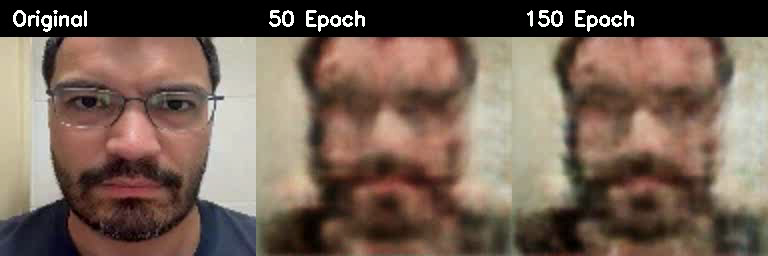
\includegraphics[width=\linewidth, height=2.1cm, keepaspectratio]{ae_vid_comp_B_to_A.png} \\
            \vspace{0.05cm}
            \scriptsize \textit{Comparison B $\to$ A (Input $\mid$ 50ep $\mid$ 150ep)}

            \vspace{0.1cm}
            \href{videos/comparison_B_to_A.mp4}{\scriptsize \underline{\textcolor{primaryNavy}{[comparison\_B\_to\_A.mp4]}}}

            \vspace{0.15cm}
            \begin{block}{Key Takeaway}
                \scriptsize
                Possible cause: the shared latent code entangled identity with facial pose and expression. This was not tested separately.
            \end{block}
        \end{column}
    \end{columns}
\end{frame}

